
\chapter{Lezione 8}
\section{Energia potenziale elettrica.}

Utilizziamo le tecniche del precorso sul lavoro e sull'energia, per studiare la forza elettrica (forza di Coulomb), che scopriremo essere conservativa
\begin{figure}[h]
	\begin{center}
		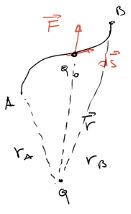
\includegraphics[width=4cm]{lezione8/images/1 Elettrostatica, Il potenziale elettrico}\\
		\caption{Situazione schematizzata per il calcolo dell'energia potenziale di una carica puntiforme}
	\end{center}
\end{figure}

Supponiamo di avere una carica puntiforme $q$ positiva (per convenzione) e studiamo il lavoro che questa carica fa su una carica test $q_0$ per spostarla da un punto A ad un punto B. In ogni istante infinitesimo avremmo una forza del tipo 
$$\vec{F}=k_e \frac{qq_0}{r^2}\frac{\vec{r}}{r}$$
Quindi calcoliamo il lavoro
$$\vec{F}\cdot d\vec{s}=k_e  \frac{qq_0}{r^2}\frac{\vec{r}}{r}d\vec{s}$$
Se vediamo da vicino quello che sta acccadendo in un determinato momento possiamo rappresentare le forze e gli spostamenti come segue

\begin{figure}[h]
	\begin{center}
		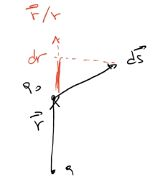
\includegraphics[width=4cm]{lezione8/images/2 Elettrostatica, Il potenziale elettrico}\\
		\caption{Ingrandimento situazione schematizzata in precedenza}
	\end{center}
\end{figure}

Di conseguenza 
$$ k_e \frac{qq_0}{r^2}\frac{\vec{r}}{r}d\vec{s}=k_e \frac{qq_0}{r^2}dr$$
Allora possiamo calcolare il lavoro
$$L_{AB}=\int_{A}^{B}\vec{F}\cdot d\vec{s}=k_e \int_{A}^{B}\frac{qq_0}{r^2}dr=\left[ -k_e \frac{qq_0}{r}\right] _A ^B = k_e \frac{qq_0}{r_A}-k_e \frac{qq_0}{r_B}=E_p (A)-E_p(B)$$.

Quindi la forza elettrica è una forza conservativa.

In generale l'espressione dell'energia potenziale in un punto $q_0$ a distanza $r$ da $q$ è data da 
$$E_p (r) =k_e \frac{qq_0}{r}$$

\begin{figure}[h]
	\begin{center}
		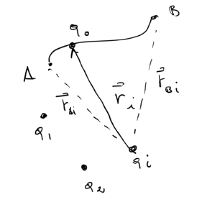
\includegraphics[width=4cm]{lezione8/images/3 Elettrostatica, Il potenziale elettrico}\\
		\caption{Potenziale di più cariche puntiformi}
	\end{center}
\end{figure}

Da qui possiamo andare a calcolare il potenziale di una distribuzione di carica qualsiasi calcolando 
$$\int_{A}^{B}\vec{F_i}\cdot d\vec{s}=k_e \int_{A}^{B}\frac{q_i q_0}{r^2}dr = k_e \frac{q_i q_0}{r_{A_i}}-k_e \frac{qq_0}{r_{B_i}}$$ 
e ricordando che 
$$\int_{A}^{B}\vec{F}\cdot d\vec{s}=\int_{A}^{B}\sum_{i=1}^{n}\vec{F_i}\cdot d\vec{s}=\sum_{i=1}^{n}\int_{A}^{B}\vec{F_i}\cdot d\vec{s}=\sum_{i=1}^{n} \left[ E_{p_i}(A)-E_{p_i}(B)\right] $$

Notiamo che se il potenziale nel punto B è zero possiamo parlare di energia potenziale nel punto A, e per farlo possiamo pensare sempre che vogliamo spostare una carica dal punto A all'infinito, per fare in modo che nel punto B l'energia potenziale si annulli. (trucco)
\section{Potenziale elettrico}

Analogamente al quanto visto per il campo elettrico definiamo 

\begin{definizione}[Potenziale elettrico]
	Il potenziale elettrostatico è definito come 
	$$V(r)=\frac{E_p (r)}{q_0}$$
\end{definizione}
\begin{itemize}
	\item E' una funzione solamente della distanza/posizione
    \item E' definito a meno di una costante additiva arbitraria, cioè ciò che ha significato fisico non è il valore in se, ma le differenze di potenziale elettrico.
    \item L'unità di misura è $\frac{J}{C}=V$ (volt).
\end{itemize}

\begin{esempio}[cariche puntiformi]
Abbiamo calcolato per le cariche puntiformi l'energia potenziale, da cui possiamo ottenere $$V(r)=\sum_{i=1}^{n} \dfrac{E_{p_i} (r)}{q_0}$$
\end{esempio}
\subsection{Relazione tra $\vec{E}$ e V}
Questa relazione è relazionata alla nozione di energia potenziale. Infatti abbiamo già visto che 

$$L_{AB}=\int_{A}^{B}q_0 \vec{E} \cdot d\vec{s}= q_0 \left[V(A)-V(B) \right] $$
Se ci liberiamo di $q_0$ otteniamo semplicemente l'espressione 
$$\int_{A}^{B}\vec{E} \cdot d\vec{s}= V(A)-V(B)= \int_{A}^{B}(-dV)$$

Da cui possiamo ottenere la relazione 

$$-\vec{E} \cdot d\vec{s}=  dV$$

\begin{esempio}(dipolo elettrico)
	
	\begin{figure}[h]
		\begin{center}
			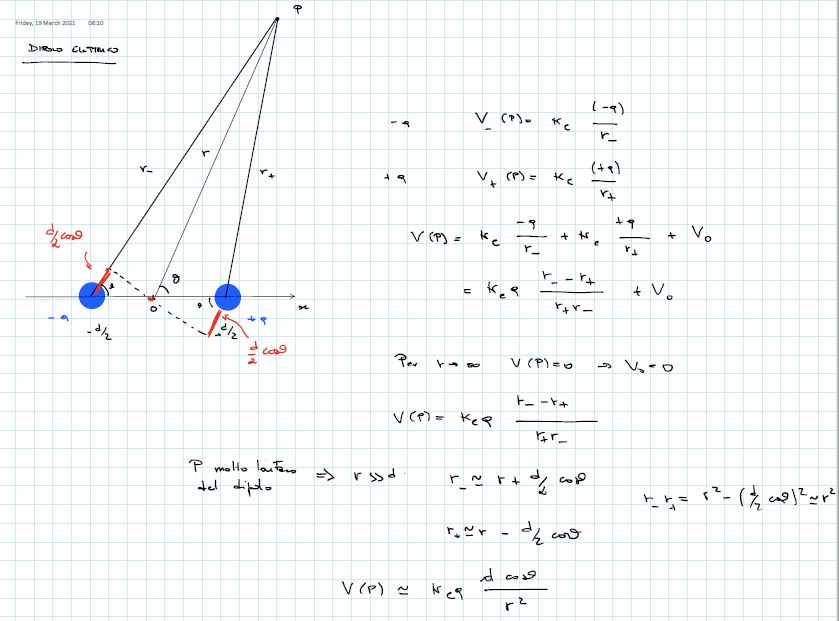
\includegraphics[width=15cm]{lezione8/images/4 Elettrostatica, Il potenziale elettrico}\\
			\caption{Calcolo del potenziale del dipolo elettrico}
		\end{center}
	\end{figure}

Dove $p=qd$ lo avevamo chiamato \textit{momento del dipolo}. Perciò
$$V(r)=k_e \frac{\vec{p}\cdot \vec{u_r}}{r^2}$$
\end{esempio}


\clearpage
\begin{esempio}(distribuzione continua)
		\begin{figure}[h]
		\begin{center}
			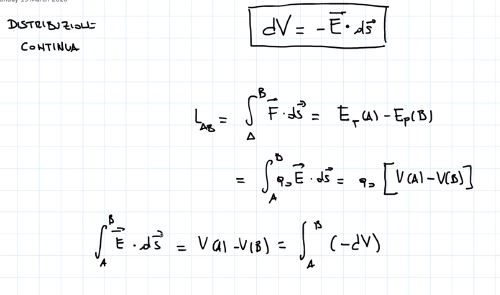
\includegraphics[width=12cm]{lezione8/images/5 Elettrostatica, Il potenziale elettrico}\\
			\caption{Potenziale di una distribuzione continua generale}
		\end{center}
	\end{figure}
\end{esempio}
\clearpage
\begin{esempio}(distribuzione piana uniforme)
	\begin{figure}[h]
	\begin{center}
		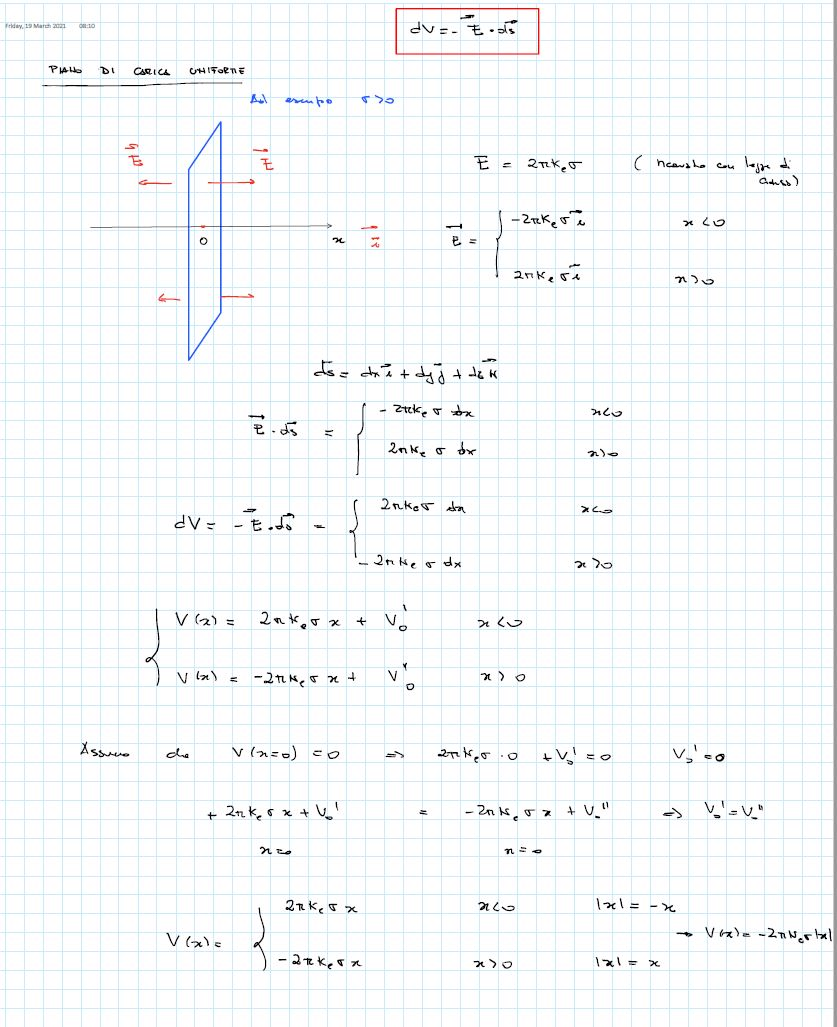
\includegraphics[width=13cm]{lezione8/images/6 Elettrostatica, Il potenziale elettrico}\\
		\caption{}
	\end{center}
\end{figure}
\end{esempio}
\clearpage
\begin{esempio}(sfera uniformemente carica)
	\begin{figure}[h]
	\begin{center}
		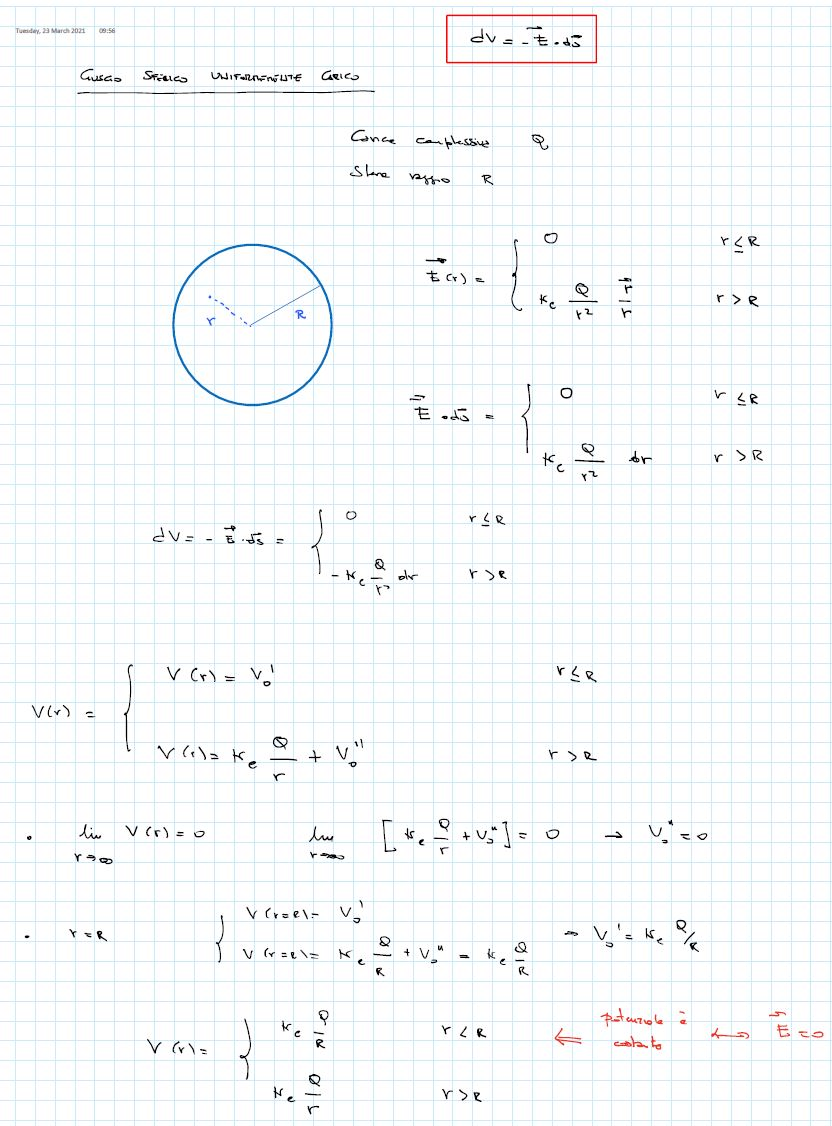
\includegraphics[width=11cm]{lezione8/images/9 Elettrostatica, Il potenziale elettrico}\\
		\caption{}
	\end{center}
\end{figure}
	
\end{esempio}
\clearpage
Quindi fino ad ora abbiamo calcolato potenziali dalla relazione $dV=-\vec{E}\cdot d\vec{s}$ una volta noto il campo elettrico. Possiamo allora chiederci se esista una relazione opposta da cui noto il potenziale, possiamo calcolare il campo elettrico

	\begin{figure}[h]
	\begin{center}
		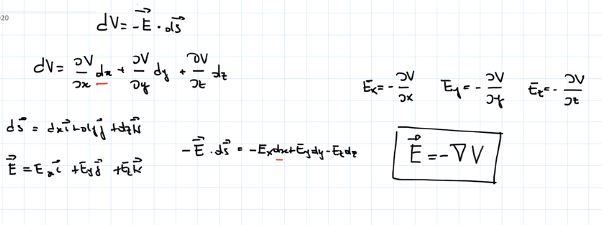
\includegraphics[width=10cm]{lezione8/images/12 Elettrostatica, Il potenziale elettrico}\\
		\caption{Espressione del campo elettrico in funzione del potenziale}
	\end{center}
\end{figure}

\begin{definizione}[superficie equipotenziali]
	Una superficie si dice equipotenziale se ogni punto su di esso si trova allo stesso potenziale
\end{definizione}

	\begin{figure}[h]
	\begin{center}
		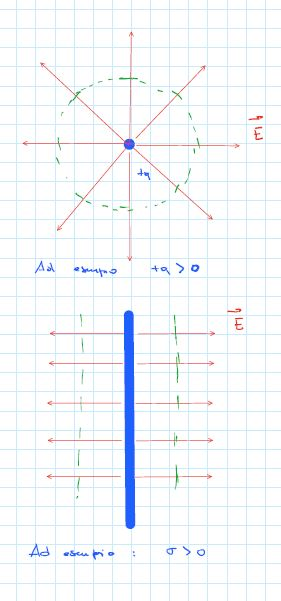
\includegraphics[width=4cm]{lezione8/images/13 Elettrostatica, Il potenziale elettrico}\\
		\caption{Esempi di alcuni superficie equipotenziali, sferica nel caso a sinistra e piana nel caso a destra}
	\end{center}
\end{figure}


Quindi se riassumiamo 
\begin{itemize}
\item abbiamo scoperto che la forza di Coulomb è una forza conservativa e perciò gli possiamo associare un energia potenziale (calcolata in diverse occasioni)
\item in analogia al passaggio da forza di Coulomb e campo elettrico, possiamo introdurre il potenziale
\item per il campo elettrico si era enunciato il principio di sovrapposizione, in questo caso possiamo sommare i potenziali, possiamo chiamare questo fatto come \textit{Principio di additività} 
\end{itemize}

\begin{figure}[h]
	\begin{center}
		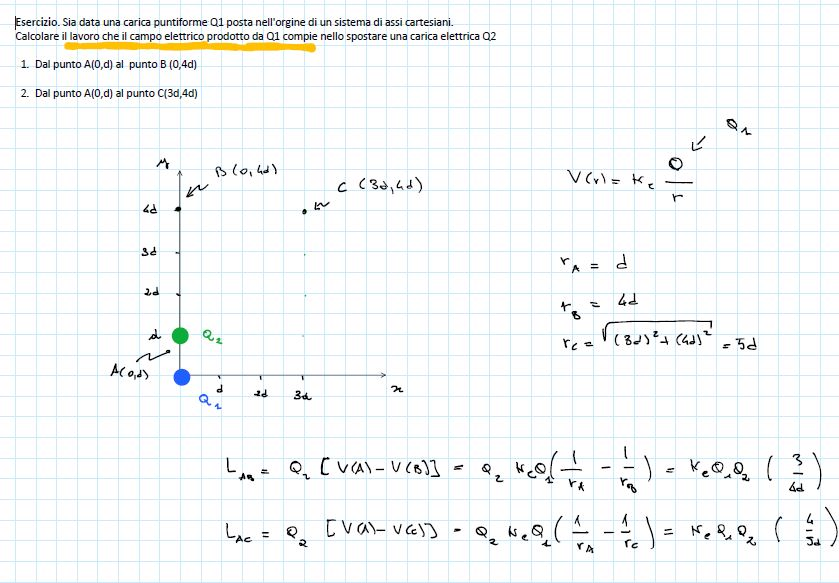
\includegraphics[width=12cm]{lezione8/images/14 Elettrostatica, Il potenziale elettrico}\\
		\caption{Esercizio proposto}
	\end{center}
\end{figure}
